% Appendix A

\chapter{Appendix}\label{ch:appendix}

\section{Selected Reference Manual for Java Package \textbf{\emph{au.csiro.iekbase.integration}}}
\label{manual}
\begin{center}\Large
Reference Manual for Java Package \emph{Satellite Data Integration}\\
Cecil Li\\li11v@csiro.au
\end{center}
\subsection{Shared Drive directory structure}
Shared drive remote path
\begin{quote}\begin{verbatim}  
	\\fstas1-hba.nexus.csiro.au\ICT-SHARE\Ict Groups\Tasmanian ICT Centre\
\end{verbatim}\end{quote}
Local Machine mappping Path, e.g.
\begin{quote}\begin{verbatim}  
Z:\
\end{verbatim}\end{quote}
Detailed directory structure

\begin{quote}
\begin{lstlisting}  
ls Z:\LandSAT Data
  \Digital Elevation Data
    \1sSRTM_2008_DEMs_ESRI_GRID_1sx1s_Mosaic
        - Uncompressed raw data folder from National Elevation Data Framework(NEDF) Portal
        - 1 second resoltuion, in ESRI-GRID format
    australia.tif
      - Converted GeoTIFF file of Tasmania
    AWAPmapping.csv
      - Generated Mapping file of AWAP to DED resolution
    MODISmapping.csv
      - Generated Mapping file of MODIS to DED resolution
    output.csv
      - Generated DED data file of the selected region with given lat,lon,width and height of the rectangle area
  \Examples
    - Contains example of LandSAT images, in compressed jpeg format
  \LandSAT ETM+ SLC-OFF
    - LandSAT 7 raw data, with the SLC OFF
    - Dates from 2010 to 2013
  \LandSAT ETM+ SLC-ON
    - LandSAT 7 raw data, with the SLC ON
    - Dates from 2000 to 2003
  \LandSAT Low Res Previews
    - Contains compressed jpeg format images for preview
  \LandSAT OLI-TIRS
    - LandSAT 8 raw data
    - Dates from 2013 onwards
  \LandSAT TM
    - LandSAT 4-5 raw data
    - Dates from 1987 to 1999 and 2003 to 2009
  \Metafiles
    - Contains metafiles used for submitting bulk download orders
  \MODIS Output
    - Contains weekly folders, with naming convention YYYYMMDD-YYYYMMDD, of which the starting date is a Monday
    \20070129-20070204
      - Example weekly folder, where 29th Jan 2007 is a Monday and 4th Feb 2007 is the following Sunday
      AWAPoutput.csv
        - Region Data from the AWAP dataset saved in .csv format
      MODISoutput.csv
        - Region Data from the MODIS dataset saved in .csv format
      WaterBalanceoutput.csv
        - Region Data of the water balance model calculated using AWAPoutput.csv , saved in .csv format
    \...
  \MODIS Sample
    - Contains a few of the MODIS VI product sample files, in .hdf format
  \MODIS VI
    - Contains all MODIS VI data files, both Aqua and Terra products.
    - Dates from 2000 to current time, with an 8 days gap.
  bulk download application.exe
    - An application that provided by US. Geological Survey(USGS) to download processed bulk orders
  Point_of_Interest_Marked_on_LandSAT_P90_R90_Houston_Farm.jpg
    - Screenshot of the LandSAT tile P90 R90, which is the south-eastern Tasmania
  USGS_P90_R90_LandSAT_TasTile_Cover_Houston_Farm.jpg
    - Screenshot of all the LandSAT tiles that covers Tasmania
	\end{lstlisting}
\end{quote}
\subsection{Download DED data}
How to download DED data for the region of interest?
\begin{enumerate}
\item
Access the National Elevation Data Framework(NEDF) Portal on\\
	\href{http://nedf.ga.gov.au/geoportal/catalog/main/home.page}{http://nedf.ga.gov.au/geoportal/catalog/main/home.page}

\item
Register a free account or use existing account to login.
\item
Access to the search page on \\
\href{http://nedf.ga.gov.au/geoportal/catalog/search/search.page}{http://nedf.ga.gov.au/geoportal/catalog/search/search.page}

\item
Use the "Select" tool above the map on the left panel, choose the region that is of interest. Parameters of the selected region will be automatically shown on the "State" section on the right panel.\\
Type in \emph{1sSRTM} in the keyword textbox so that the search results are limiting to 1 second resolution of SRTM products. Then click the "Search" button on top of the right panel, a list of available products will be shown, choose the one with ''DEMs'' for Digital Elevation Model.
	\begin{figure}[H]\begin{center}
	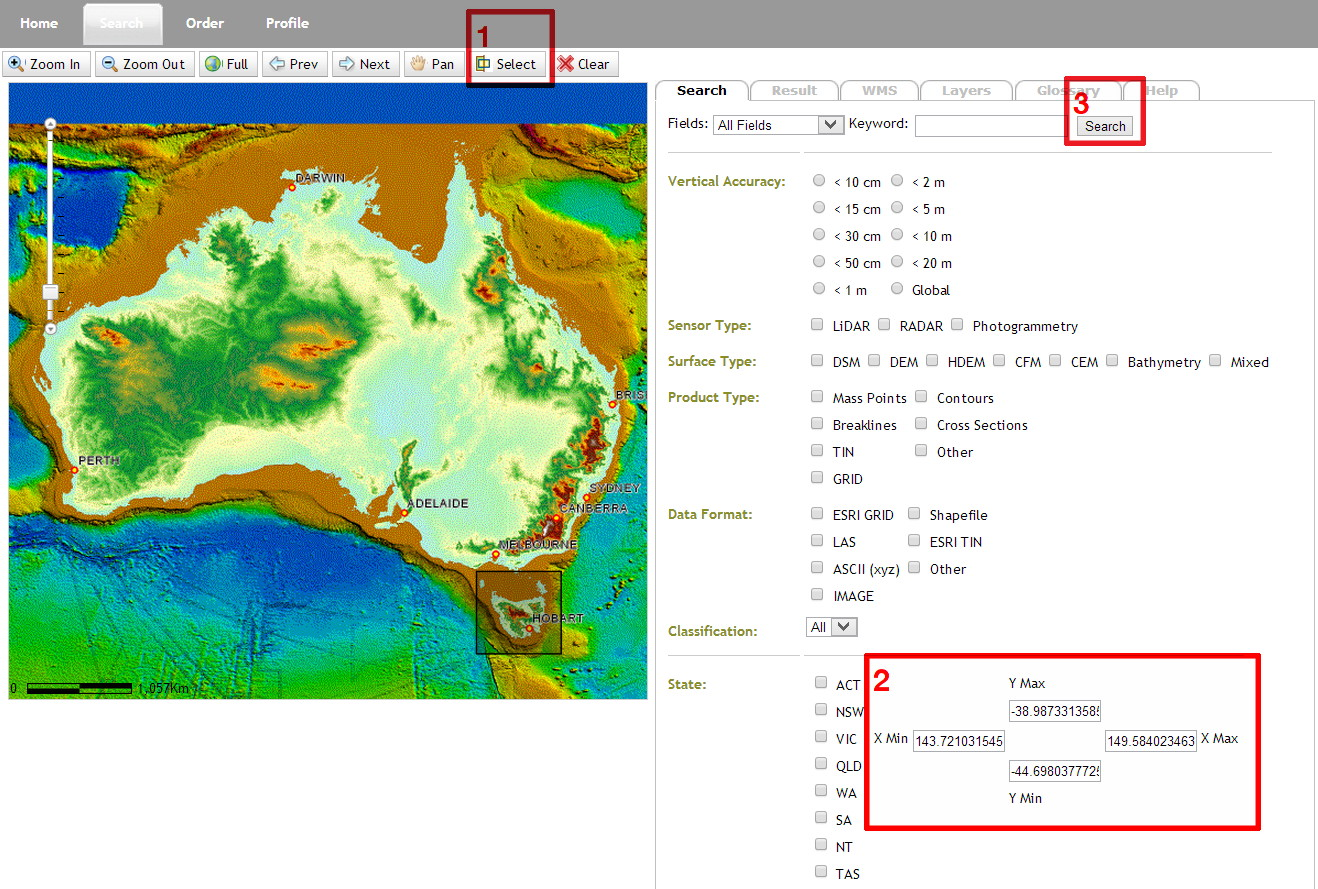
\includegraphics[width=\textwidth]{gfx/appendixf1.jpg}
	\caption{Use of NEDF portal search function}
	\end{center}\end{figure}
\item
Additional parameters can also be entered on the right panel to filter out results.
\item
From the list of available products, check the checkbox for the product that suits the need and proceed by clicking the "order" button. \\
Note that there is a limit of 2GB per download order limit with the NEDF portal.
\item
An email with confirmation of order will be sent to the registered address, and it takes up to 3 business days for the order to be processed. 
After which, an email containing the download link of the data will be sent to the registered email address.

\end{enumerate}




\subsection{Download MODIS data}\label{Section:Download the MODIS data}
How to download MODIS data for the region of interest?
\begin{enumerate}
\item
Access the USGS visualized earth explorer on \href{http://earthexplorer.usgs.gov/}{http://earthexplorer.usgs.gov/}
\item
Register a free account or use existing account to login.
\item
Enter the search criteria in the left panel.
\item \label{Step:select dataset}
In the "Data Sets" tab, collapse on "NASA LPDAAC Collections", then collapse on "MODIS Vegetation Indices", make sure the checkboxes for \textbf{"MODIS MOD13Q1" or "MODIS MYD13Q1"} are checked. Then click "Results" button.
\item
Click the button next to "export your results", select "Comma Delimited" as the export format, and click "Export".
\begin{figure}[H]\begin{center}
	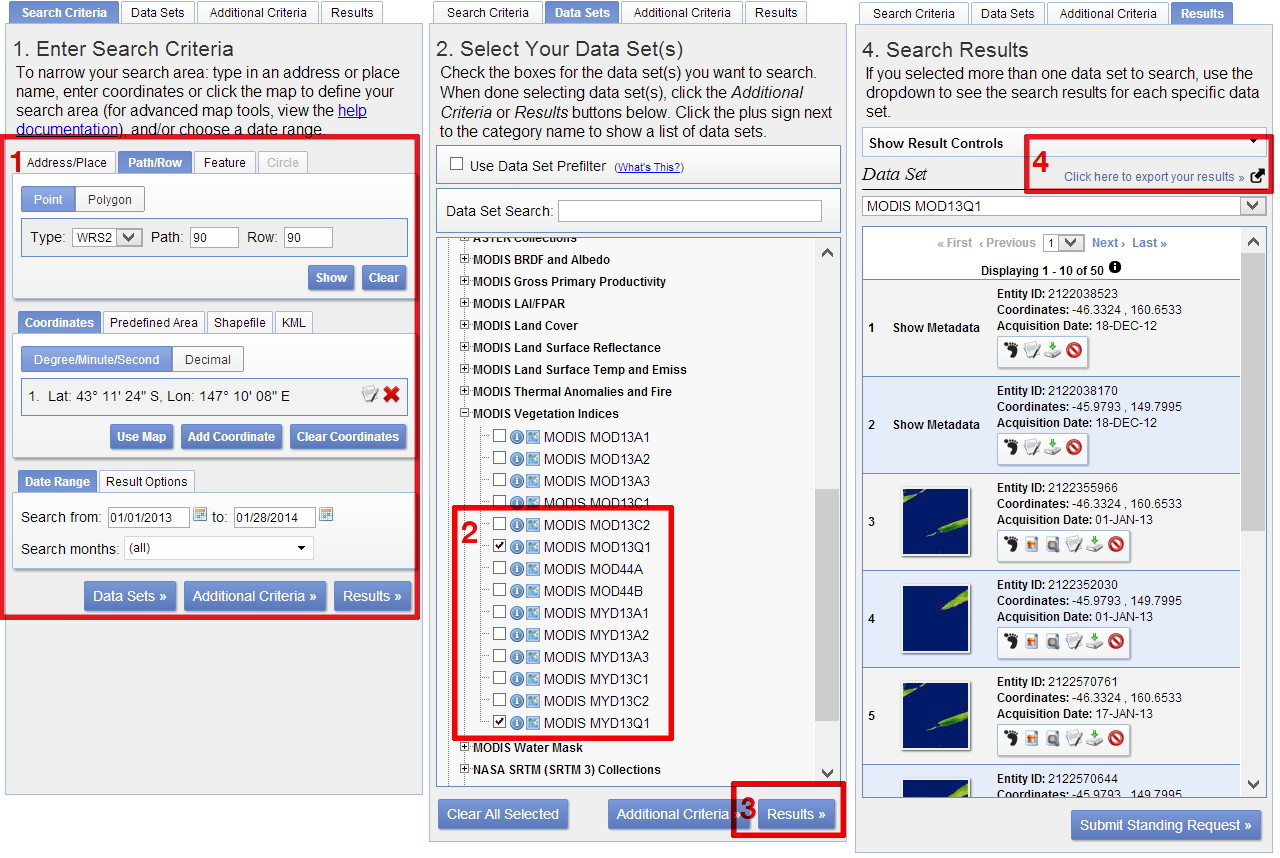
\includegraphics[width=\textwidth]{gfx/appendixf2.jpg}
	\caption{Use of USGS earth explorer}
\end{center}\end{figure}
\item
An email containing the metadata download link will be sent to the registered email address.\\ Download the metadata, uncompress to get a textfile.
\item
Access the bulk download order page on \href{http://earthexplorer.usgs.gov/filelist/}{http://earthexplorer.usgs.gov/filelist/}
\item
Choose the downloaded metadata file, find the desired dataset in the drop-down list and then click "Submit File List".
\item
Select "Standard format" in the download products section and submit the order.
\item
A confirmation email of submitted order will be sent to the registered email address, which also provides a link to the Bulk Download Application.
\item
Install the BDA, open and login with USGS account credentials. A list of current orders will be shown in the window.
\item
Choose the order that is of interest, make sure the save folder is correct then click the download button.\\
It should start the download process automatically.
\end{enumerate}
\subsection{Download Landsat data}\label{Section:Download Landsat data}
How to download Landsat data for the region of interest?\\
\newline
Similar to Section \ref{Section:Download the MODIS data}, the Landsat data are available from the USGS earth explorer portal. Only this time, in Step \ref{Step:select dataset}, choose the dataset from \emph{Landsat Archive}, select the one that suits the time requirement and bandwidth definition following the information in Table \ref{Table:landsat}.
\begin{center}
\begin{table}[H]
\small
\begin{tabular}{ | p{1.2cm}| >{$}p{2.2cm}<{$} | >{$}p{2.8cm}<{$} | >{$}p{2.2cm}<{$}| >{$}p{2.8cm}<{$}| >{$}p{2.2cm}<{$}|}
    \hline
    Time & 1987-1999 & 2000-2003 & 2003-2009 & 2010-2013 & 2013-Now \\ \hline
    Landsat & \text{L5 TM} & \text{L7 ETM+ SLC-ON} & \text{L5 TM}& \text{L7 ETM+ SLC-OFF} & \text{L8 OLI-TIRS} \\ \hline
    Band 1 & 0.45-0.52\mu m &0.45-0.52\mu m& 0.45-0.52\mu m& 0.45-0.52\mu m & 0.43-0.45\mu m\\ \hline
	Band 2&0.52-0.60\mu m&0.52-0.60\mu m&0.52-0.60\mu m&0.52-0.60\mu m&0.45-0.51\mu m\\ \hline
	Band 3&0.63-0.69\mu m&0.63-0.69\mu m&0.63-0.69\mu m&0.63-0.69\mu m&0.53 - 0.59\mu m\\\hline
	Band 4&0.76-0.90\mu m&0.76-0.90\mu m&0.76-0.90\mu m&0.76-0.90\mu m&0.64-0.67\mu m \\\hline
	Band 5&1.55-1.75\mu m&1.55-1.75\mu m&1.55-1.75\mu m&1.55-1.75\mu m&0.85-0.88\mu m \\\hline
	Band 6&10.40-12.50\mu m&10.40-12.50\mu m&10.40-12.50\mu m&10.40-12.50\mu m&1.57-1.65\mu m \\\hline
	Band 7&2.08-2.35\mu m&2.09-2.35\mu m&2.08-2.35\mu m&2.09-2.35\mu m&2.11-2.29\mu m\\ \hline
	Band 8&n/a&0.52-0.90\mu m&n/a&0.52-0.90\mu m&0.50-0.68\mu m\\\hline
	Band 9&n/a&n/a&n/a&n/a&1.36-1.38\mu m\\ \hline
	Band 10&n/a&n/a&n/a&n/a&10.60-11.19\mu m\\ \hline
	Band 11&n/a&n/a&n/a&n/a&11.50-12.51\mu m\\ \hline
\end{tabular}
\begin{tabular}{ |  p{1.2cm} |p{2.2cm} | p{2.8cm}| p{2.2cm}| p{2.8cm}|p{2.2cm}|}
	Note & & & Data missing for some periods & Image are defected due to SLC failure & Very Large Data files\\
	\hline
\end{tabular}
\caption{Landsat Products Specification}\label{Table:landsat}
\end{table}
\end{center}
The BDA will download the landsat data in a folder, each weekly file is compressed in a tar.gz, which should be uncompressed to a .tar, which then be compressed in its own folder such as LT5XXXXXXXXXXX ,within that folder, there will be multiple band files in GeoTif format and a metadata file with \_MTL.txt as extension.


\subsection{Use Satellite Data Integration Package in Eclipse}
Required software packages:
\begin{itemize}
\item
Eclipse Juno+
\item
Subversion
\item
HDF-java\\
Download the binary for corresponding OS at \\
		\href{http://www.hdfgroup.org/products/java/release/download.html}{http://www.hdfgroup.org/products/java/release/download.html}
\item
m2eclipse plug-in\\
In Eclipse, click Help-Install New Software-Enter the following link\\
\href{http://download.eclipse.org/technology/m2e/releases}{http://download.eclipse.org/technology/m2e/releases}
\end{itemize}
Checkout SVN repo:
\begin{quote}\begin{lstlisting}
https://svnserv.csiro.au/svn/issl-repo/iekbase/source/Intelligent_Mobile_Application_Sustainable_Irrigation_Water_Usage_DSS/
\end{lstlisting}\end{quote}
In Eclipse,
\begin{itemize}
\item
Import existing project "CosmOz".
\item
Import existing maven project "Satellite Data Integration" and "Graphic Demo" (optional)
\item
Right-click on the imported Maven project and select Maven-Update Projects, then Eclipse would download all the dependencies to the local machine.
\item
Uncompress the downloaded HDF-java package in the local machine and add the \textbackslash hdf-java\textbackslash  lib to the Java Build Path for package "Satellite Data Integration"
\item
Create a textfile named "sample.config" with the following parameters. Put it in the svn root folder, namely
\\"Intelligent\_Mobile\_Application\_Sustainable\_Irrigation\_Water\_Usage\_DSS"
\end{itemize}
\begin{quote}
\begin{lstlisting}  
app.name=Satellite Data Integration
app.version=1.0

app.dataset=MODIS
app.dataset2=AWAP
MODIS.datafolder=Z:/LandSAT Data/MODIS VI
MODIS.savefolder=Z:/LandSAT Data/MODIS Output

geo.latitude = -42.695749
geo.longitude = 147.512746
geo.width = 20
geo.height = 20

time.startTime = 2000000
time.endTime = 2014999
DED.datapath=Z:/LandSAT Data/Digital Elevation Data/Australia.tif
DED.savepath=Z:/LandSAT Data/Digital Elevation Data/output.csv

MAPPING.pathMODIS=Z:/LandSAT Data/Digital Elevation Data/MODISmapping.csv
MAPPING.pathAWAP=Z:/LandSAT Data/Digital Elevation Data/AWAPmapping.csv


AWAP.datafolder = C:/Users/li11v/Intelligent_Mobile_Application_Sustainable_Irrigation_Water_Usage_DSS/res/CosmOz
AWAP.savefolder = Z:/LandSAT Data/MODIS Output


WaterBalance.savefolder = Z:/LandSAT Data/MODIS Output
Landsat.datafolder  = Z:/LandSAT Data/Landsat TM/
Landsat.savefolder = Z:/LandSAT Data/MODIS Output
\end{lstlisting}
\end{quote}

\subsubsection{Set up the data folder for a location}
\begin{enumerate}
\item
Create the Folder, e.g. F:\textbackslash Data\textbackslash LocationA\\
\item
Create a .config file following the given sample for the executable jar, put it in the parent folder of the executable
\item
Make sure the folder path in the config file is correct, with / instead of \textbackslash on every occurrence.
\item
Run the jar in command-line as shown in section \ref{Section:Using the Runnable Jar}.
\item
Following this order when processing datasets
	\begin{enumerate}
	\item
	DED\_parser
	\item
	AWAP\_parser
	\item
	MODIS\_batch
	\item
	Landsat\_batch (In progress)
	\item
	WaterBalanceAWAP
	\item
	MappingGenerator	
	\end{enumerate}
\end{enumerate}
\subsubsection{Using the Runnable Jar}\label{Section:Using the Runnable Jar}
The executable jar is located in \textbackslash Executable folder, namely \emph{IntegrationExecutable.jar}, To run the executable, follow the manner as detailed below.\\
\newline
In command line, browse to the \textbackslash Executable folder, type in command\\
\begin{quote}
\begin{lstlisting}
F:\Intelligent_Mobile_Application_Sustainable_Irrigation_Water_Usage_DSS\Executable>java -jar -Xmx1024m IntegrationExecutable.jar -run CLASSNAME
\end{lstlisting}
\end{quote}
Where CLASSNAME is one of the following
\begin{quote}
\begin{lstlisting}
AWAP_parser, DED_parser, MappingGenerator, WaterBalanceAWAP, Landsat_parser, MODIS_batch, MODIS_parser, MODIS_reprojecton
\end{lstlisting}
\end{quote}
Note that, for \emph{MODIS}, a specific VM argument is required.
\begin{quote}
\begin{lstlisting}
>java-Xmx1024m -Djava.library.path="C:\Program Files\HDF_Group\HDF-JAVA\2.10.0\lib" -jar IntegrationExecutable.jar -run MODIS_batch
\end{lstlisting}
\end{quote}
Where the exact folder should be according to your local installation of the HDF-java package\\
\newline
Below explains the function of each runnable class. 
\begin{quote}
\begin{lstlisting}
  AWAP_parser
    - Extract the region values defined by geo.* in the config file, from "AWAP.datafolder" and save to "AWAP.savefolder" in a weekly manner.
  DED_parser
    - Extract the region values defined by geo.* in the config file, from the file "DED.datapath" and save to the file "DED.savepath" in .csv format.
  MappingGenerator
    - Generates mapping file from low resolution dataset to high resolution, the DED. Reads parameters "MODIS.savefolder", "DED.savepath", "waterBalance.savefolder" for reading data, as well as "MAPPING.pathMODIS" and "MAPPING.pathAWAP" for saving output file in .csv format.
  WaterBalanceAWAP
    - Calculates the region values using water balance model, from the AWAP output weekly data which are saved in "AWAP.savefolder". Saved in the weekly folders under "WaterBalance.savefolder".
  MODIS_batch
    - Extract the region values defined by geo.* in the config file, from "MODIS.datafolder" where all the *.hdf are stored and save to "MODIS.savefolder" in a weekly manner.
  Landsat_batch
    - Extract the region values defined by geo.* in the config file, from "Landsat.datafolder" where all the *.TIF are stored and save to "Landsat.savefolder" in a weekly manner.
\end{lstlisting}
\end{quote}


%----------------------------------------------------------
\newpage
\section{Sample: JSON file for transmission from the web interface to the Android application}
\label{JSONsample}
\begin{quote}
\begin{lstlisting}
{"header":{
	"Version":"1.0",
	"Last Update":"20130114"},
"body":{
	"Locations":
	["Baldry","Daly River","Gnangara","Griffith","Norwin","Robson Ck Single Tube","Robson Ck Dual Tube","Tullochgorum","Tumbarumba","Weany Ck","Yanco"],
	"Latitude":
	[-32799999,-14200000,-31400000,-29500000,-27600000,-17100000,
	-17100000,-41700000,-35700000,-19900000,-35000000],
	"Longitude":
	[148500000,131400000,115700000,149500000,151300000,145600000,
	145600000,147900000,148200000,146500000,146300000],
	"Elevation":
	[438,75,50,127,361,715,715,285,1200,287,124],
	"Land Cover":
	["Reforested & Pasture","Tropical Savannah","Banksia Woodland","Irrigated Pumpkins","Cotton","Rainforest","Rainforest","Improved Pasture","Wet Sclerophyll Eucalypt Forest","Open woodland, shrubby understory","Open Grassland"],
	"Land Use":
	["Grazing","Grazing","National Park/State Forest","Agriculture","Agriculture","World Heritage Protected Area","World Heritage Protected Area","Grazing","Native/Plantation Forestry","Grazing","Grazing, Irrigated Cropping"],
	"date":
	["30/03/2011","7/06/2011","11/05/2011","1/10/2011",
	"30/03/2011","28/10/2010","19/09/2011","15/12/2010",
	"3/04/2011","1/12/2010","1/04/2011"],
	"Indicators":
	[2,2,2,1,1,2,2,2,2,2,2],
	"Confidence":
	[0.1,0.2,0.3,0.4,0.5,0.6,0.7,0.8,0.9,1.0,1.1]
	}
}
\end{lstlisting}
\end{quote}
%-------------------------
\newpage
\section{List Of Java Classes}\label{listofjava}
\begin{quote}
\begin{lstlisting}
au.csiro.iekbase.cosmoz
	ASRISProcessor.java
	AWAP_Preprocessor.java
	BOM_Webdata_Batch_Preprocessor.java
	BPNN.java
	CosmOz_Data_Preprocessor.java
	CsvReader.java
	CsvWriter.java
	FTPDownload.java
	generalMethods.java
	LDA.java
	LinearInterpolation.java
	MAIN.java
	MultiDataIntegration.java
	SILO_Data_Preprocessor.java
	SOM_Class1.java
	SOM.java
au.csiro.iekbase.graphicDemo
	CustomColorMap.java
	DEDreader.java
	MAPreader.java
	MODISreader.java
	ScatterPlot.java
	SurfacePlot.java
	TitleRenderer.java
au.csiro.iekbase.awap
	AWAP_parser.java
	AWAP_parserTest.java
	WaterBalanceAWAP.java
	WaterBalanceAWAPTest.java
au.csiro.iekbase.digitalElevationData
	DED_parser.java
	DED_parserTest.java
au.csiro.iekbase.integration
	Initialization.java
	IntegrationExecutable.java
	MappingGenerator.java
	MappingGeneratorTest.java
au.csiro.iekbase.landsat
	Landsat_batch.java
	Landsat_parser.java
	Landsat_batchTest.java
	Landsat_parserTest.java
au.csiro.iekbase.modis
	MODIS_batch.java
	MODIS_batchTest.java
	MODIS_parser.java
	MODIS_parserTest.java
	MODIS_reprojection.java
	MODIS_reprojectionTest.java
au.csiro.iekbase.android
	MainActivity.java
au.csiro.iekbase.water
	Water.java
au.csiro.iekbase.waterGUI
	Main.java
	TextAreaOutputStream.java
au.csiro.iekbase.web.controllers
	Application.java
	Metadata.java
au.csiro.iekbase.wrapper
	Wrapper.java
\end{lstlisting}
\end{quote}
%-------------------------
\newpage
\section{List Of MATLAB Scripts}\label{listofmatlab}
\begin{quote}
\begin{lstlisting}
analysis_MODIS_Landsat.m
ANFIS_for_High_Res.m
arrow.m
csvimport.m
estimatedWBfromVI.m
extractWaterDEDMODIS.m
mapToHighRes.m
mapToLowRes.m
MODIS_AWAP_WB_mLearning.m
normalizeDATA.m
Performance_Eval.m
plotAWAP.m
plotAWAP_FitDistribution.m
plotDED.m
plotEnhancedWB.m
plotWB.m
rdir.m
readAWAP.m
readDED.m
readLANDSAT.m
readMODIS.m
readWB.m
test.m
\end{lstlisting}
\end{quote}